\documentclass[preprint]{sigplanconf}

\usepackage{graphicx}
\usepackage{comment}
\usepackage{amsmath}
\usepackage{xspace}
\usepackage{amssymb}
\usepackage{stmaryrd}
\usepackage{proof}
\usepackage{multicol}
\usepackage[nodayofweek]{datetime}
\usepackage{etex}
\usepackage[all, cmtip]{xy}
\usepackage{xcolor}
\usepackage{listings}
\usepackage{multicol}
\newcommand\hmmax{0} % default \newcommand\bmmax{0} % default 4
\usepackage{bm}
\usepackage{cmll}

\newcommand{\fname}[1]{\ulcorner #1 \urcorner}
\newcommand{\fconame}[1]{\llcorner #1 \lrcorner}

\newcommand{\xcomment}[2]{\textbf{#1:~\textsl{#2}}}
\newcommand{\amr}[1]{\xcomment{Amr}{#1}}
\newcommand{\roshan}[1]{\xcomment{Roshan}{#1}}

\newcommand{\asterix}[0]{*}

\newcommand{\ie}{\textit{i.e.}\xspace}
\newcommand{\eg}{\textit{e.g.}\xspace}

\newcommand{\lcal}{\ensuremath{\lambda}-calculus\xspace}
\newcommand{\G}{\ensuremath{\mathcal{G}}\xspace}

\newcommand{\code}[1]{\lstinline[basicstyle=\small]{#1}\xspace}
\newcommand{\name}[1]{\code{#1}}

\def\newblock{}

\newenvironment{floatrule}
    {\hrule width \hsize height .33pt \vspace{.5pc}}
    {\par\addvspace{.5pc}}

\newtheorem{theorem}{Theorem}[section]
\newtheorem{lemma}[theorem]{Lemma}
\newtheorem{definition}[theorem]{Definition}
\newtheorem{proposition}[theorem]{Proposition}
\newenvironment{proof}[1][Proof.]{\begin{trivlist}\item[\hskip \labelsep {\bfseries #1}]}{\end{trivlist}}

\newcommand{\arrow}[1]{\mathtt{#1}}

\newcommand{\dgm}[2][0.95]{
\begin{center}
\scalebox{#1}{
\includegraphics{diagrams/#2.pdf}
}
\end{center}
}

%subcode-inline{bnf-inline} name langRev
%! swap+ = \mathit{swap}^+
%! swap* = \mathit{swap}^*
%! dagger =  ^{\dagger}
%! assocl+ = \mathit{assocl}^+
%! assocr+ = \mathit{assocr}^+
%! assocl* = \mathit{assocl}^*
%! assocr* = \mathit{assocr}^*
%! identr* = \mathit{uniti}
%! identl* = \mathit{unite}
%! dist = \mathit{distrib}
%! factor = \mathit{factor}
%! eta = \eta
%! eps = \epsilon
%! eta+ = \eta^+
%! eps+ = \epsilon^+
%! eta* = \eta^{\times}
%! eps* = \epsilon^{\times}
%! trace+ = trace^+
%! trace* = trace^{\times}
%! ^^^ = ^{-1}
%! (o) = \circ
%! (;) = \fatsemi
%! (*) = \times
%! (+) = +
%! LeftP = L^+
%! RightP = R^+
%! LeftT = L^{\times}
%! RightT = R^{\times}
%! alpha = \alpha
%! bool = \textit{bool}
%! color = \textit{color}
%! Gr = G

%subcode-inline{bnf-inline} regex \{\{(((\}[^\}])|[^\}])*)\}\} name main include langRev
%! Gx = \Gamma^{\times}
%! G = \Gamma
%! [] = \Box
%! |-->* = \mapsto^{\asterix}
%! |-->> = \mapsto_{\ggg}
%! |--> = \mapsto
%! <--| = \mapsfrom
%! |- = \vdash
%! <><> = \approx
%! ==> = \Longrightarrow
%! <== = \Longleftarrow
%! <=> = \Longleftrightarrow
%! <-> = \leftrightarrow
%! ~> = \leadsto
%! -o+ = \multimap^{+}
%! -o* = \multimap^{\times}
%! -o = \multimap
%! ::= = &::=&
%! /= = \neq
%! @@ = \mu
%! [^ = \lceil
%! ^] = \rceil
%! forall = \forall
%! exists = \exists
%! empty = \epsilon
%! Pi = \Pi
%! Pi0 = \Pi^{o}
%! PiEE* = \Pi^{\eta\epsilon}_{*}
%! PiEE+ = \Pi^{\eta\epsilon}_{+}
%! PiEE = \Pi^{\eta\epsilon}
%! CatSet = \textbf{Set}
%! theseus = Theseus
%! sqrt(x) = \sqrt{#x}
%! surd(p,x) = \sqrt[#p]{#x}
%! inv(x) = \frac{1}{#x}
%! frac(x,y) = \frac{#x}{#y}
%! * = \times

%%%%%%%%%%%%%%%%%%%%%%%%%%%%%%%%%%%%%%%%%%%%%%%%%%%%%%%%%%%%%%%%%%%%%%%%%%%%%%%%
\begin{document}

\conferenceinfo{POPL'13}{}
\CopyrightYear{}
\copyrightdata{}
\titlebanner{}
\preprintfooter{}

\title{Negative and Fractional Types} 

\authorinfo{Roshan P. James}
           {Indiana University}
           {rpjames@indiana.edu}
\authorinfo{Zachary Sparks} 
           {Indiana University}
           {zasparks@indiana.edu}
\authorinfo{Jacques Carette} 
           {McMaster University}
           {carette@mcmaster.ca}
\authorinfo{Amr Sabry}
           {Indiana University}
           {sabry@indiana.edu}

\maketitle

\begin{abstract}

\end{abstract}

\category{D.3.1}{Formal Definitions and Theory}{}
\category{F.3.2}{Semantics of Programming Languages}{}
\category{F.3.3}{Studies of Program Constructs}{Type structure}

\terms
Languages, Theory

\keywords continuations, information flow, linear logic, logic programming,
quantum computing, reversible logic, symmetric monoidal categories, compact
closed categories.

%%%%%%%%%%%%%%%%%%%%%%%%%%%%%%%%%%%%%%%%%%%%%%%%%%%%%%%%%%%%%%%%%%%%%%%%%%%%%%%%
\section{Introduction}

%%%%%%%%%%%%%%%%%%%%%%%%%%%%%%%%%%%%%%%%%%%%%%%%%%%%%%%%%%%%%%%%%%%%%%%%%%%%%%%%
\section{The Core Reversible Language: {{Pi}} }
\label{sec:pi}

We review our reversible language {{Pi}}: the presentation in this
section differs from the one in our previous paper~\cite{infeffects} in two
aspects. First, we add the empty type {{0}} which is necessary to express the
additive duality. Second, instead of explaining evaluation using a natural
semantics, we give a small-step operational semantics that is more
appropriate for the connections with continuations explored in this paper.

%%%%%%%%%%%%%%%%%%%%
\subsection{Syntax and Types} 
\label{sec:pi-syntax}

Unlike the traditional situation with the $\lambda$-calculus, in {{Pi}},
there is a sharp distinction between data and programs. 

\paragraph*{Data.} The sets of values and their types include:
%subcode{bnf} include main
% value types, b ::= 0 | 1 | b + b | b * b 
% values, v ::= () | left v | right v | (v, v)
Types include the empty type {{0}}, the unit type {{1}}, sum types {{b1+b2}},
and products types {{b1*b2}}.  Values includes {{()}} which is the only value
of type {{1}}, {{left v}} and {{right v}} which inject {{v}} into a sum type,
and {{(v1,v2)}} which builds a value of product type. There are no values of
type {{0}}.

\paragraph*{Programs.} All the programs of {{Pi}} are special maps of type
{{v \rightarrow v}}. Specifically, they are witnesses to the following type
isomorphisms:
%subcode{bnf} include main
%! columnStyle = r@{\hspace{-0.5pt}}c@{\hspace{-0.5pt}}l
%zeroe :&  0 + b <-> b &: zeroi
%swap+ :&  b1 + b2 <-> b2 + b1 &: swap+
%assocl+ :&  b1 + (b2 + b3) <-> (b1 + b2) + b3 &: assocr+
%identl* :&  1 * b <-> b &: identr*
%swap* :&  b1 * b2 <-> b2 * b1 &: swap*
%assocl* :&  b1 * (b2 * b3) <-> (b1 * b2) * b3 &: assocr*
%dist0 :& 0 * b <-> 0 &: factor0
%dist :&~ (b1 + b2) * b3 <-> (b1 * b3) + (b2 * b3)~ &: factor
Each line of the above table introduces one or two combinators that witness
the isomorphism in the middle. Collectively the isomorphisms state that the
structure {{(b,+,0,*,1)}} is a \emph{commutative semiring}, i.e., that each
of {{(b,+,0)}} and {{(b,*,1)}} is a commutative monoid and that
multiplication distributes over addition. The isomorphisms are extended to
form a congruence relation by adding the following constructors that witness
equivalence and compatible closure:
%subcode{proof} include main
%@  ~
%@@ id : b <-> b 
%
%@ c : b1 <-> b2
%@@ sym c : b2 <-> b1
%
%@ c1 : b1 <-> b2
%@ c2 : b2 <-> b3
%@@ c1(;)c2 : b1 <-> b3
%---
%@ c1 : b1 <-> b3
%@ c2 : b2 <-> b4
%@@ c1 (+) c2 : b1 + b2 <-> b3 + b4
%
%@ c1 : b1 <-> b3
%@ c2 : b2 <-> b4
%@@ c1 (*) c2 : b1 * b2 <-> b3 * b4

\noindent
To summarize, the syntax of {{Pi}} is given as follows. 

\begin{definition}{(Syntax of {{Pi}})}
\label{def:Pi}
We collect our types, values, and combinators, to get the full language
definition.
%subcode{bnf} include main
% value types, b ::= 0 | 1 | b+b | b*b 
% values, v ::= () | left v | right v | (v,v) 
%
% comb.~types, t ::= b <-> b
% iso ::= zeroe | zeroi 
%     &|& swap+ | assocl+ | assocr+ 
%     &|& identl* | identr* 
%     &|& swap* | assocl* | assocr* 
%     &|& dist0 | factor0 | dist | factor 
% comb., c ::= iso | id | sym c | c (;) c | c (+) c | c (*) c 
\end{definition}

\paragraph*{Adjoint.} 
An important property of the language is that every combinator {{c}} has an
adjoint {{c{dagger}}} that reverses the action of {{c}}. This is evident by
construction for the primitive isomorphisms. For the closure combinators, the
adjoint is homomorphic except for the case of sequencing in which the order
is reversed, i.e., {{(c1 (;) c2){dagger} = (c2{dagger}) (;) (c1{dagger}) }}.

\begin{definition}[Size of a type]
\label{def:size}
The size of a type {{b}}, denoted by {{[^ b ^]}}, is a numeric value
and is defined to be:
\vspace{-20pt}
\begin{multicols}{2}
%subcode{opsem} include main
% [^ b1 + b2 ^] '= [^ b1 ^] + [^ b2 ^]
% [^ b1 * b2 ^] '= [^ b1 ^] * [^ b2 ^]  

%subcode{opsem} include main
% [^ 0 ^] '= 0
% [^ 1 ^] '= 1
\end{multicols}

where {{+}} is numeric addition and {{*}} is numeric multiplication. 
  
\end{definition}
\noindent
In the setting of {{Pi}} the \emph{size}, {{[^ b ^]}}, may be simply thought of as
the number of inhabitants (an arity) of the type. This intuition will
however become tenuous in the presence of negative and fractional
types.

%%%%%%%%%%%%%%%%%%%
\subsection{Graphical Language}

The syntactic notation above is often obscure and hard to read.
Following the tradition established for monoidal
categories~\cite{springerlink:10.1007/978-3-642-12821-94}, we present
a graphical language that conveys the intuitive semantics of the
language (which is formalized in the next section).

The general idea of the graphical notation is that combinators are modeled by
``wiring diagrams'' or ``circuits'' and that values are modeled as
``particles'' or ``waves'' that may appear on the wires. Evaluation therefore
is modeled by the flow of waves and particles along the wires.

\begin{itemize}
\item The simplest sort of diagram is the {{id : b <-> b}} combinator which
  is simply represented as a wire labeled by its type {{b}}, as shown on the
  left. In more complex diagrams, if the type of a wire is obvious from the
  context, it may be omitted. When tracing a computation, one might imagine a
  value {{v}} of type {{b}} on the wire, as shown on the right.

  \begin{multicols}{2}
\begin{center}
\scalebox{0.95}{

\includegraphics{diagrams/thesis/b-wire.pdf}
}
\end{center}
\begin{center}
\scalebox{0.95}{

\includegraphics{diagrams/thesis/b-wire-value.pdf}
}
\end{center}
  \end{multicols}

\item The product type {{b1*b2}} may be represented using either one wire
  labeled {{b1*b2}} or two parallel wires labeled {{b1}} and {{b2}}. In the
  case of products represented by a pair of wires, when tracing execution
  using particles, one should think of one particle on each wire or
  alternatively as in folklore in the literature on monoidal categories as a
  ``wave.''
\begin{multicols}{2}
\begin{center}
\scalebox{0.95}{
%%subcode-line{pdfimage}[diagrams/thesis/pair-one-wire.pdf]

\includegraphics{diagrams/thesis/product-one-wire.pdf}
}
\end{center}
\begin{center}
\scalebox{0.95}{

\includegraphics{diagrams/thesis/product-one-wire-value.pdf}
}
\end{center}
\end{multicols}
\begin{multicols}{2}
\begin{center}
\scalebox{0.95}{
%%%subcode-line{pdfimage}[diagrams/thesis/pair-of-wires.pdf]
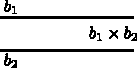
\includegraphics{diagrams/thesis/product-two-wires.pdf}
}
\end{center}
\begin{center}
\scalebox{0.95}{
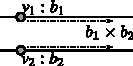
\includegraphics{diagrams/thesis/product-two-wires-value.pdf}
}
\end{center}
\end{multicols}

\item Sum types may similarly be represented by one wire or using
  parallel wires with a {{+}} operator between them. When tracing the
  execution of two additive wires, a value can reside on only one of the two
  wires.
\begin{multicols}{2}
\begin{center}
\scalebox{0.95}{
%%subcode-line{pdfimage}[diagrams/thesis/sum-one-wire.pdf]

\includegraphics{diagrams/thesis/sum-one-wire.pdf}
}
\end{center}
\begin{center}
\scalebox{0.95}{
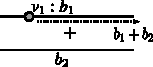
\includegraphics{diagrams/thesis/sum-two-wires-left-value.pdf}
}
\end{center}
\end{multicols}
\begin{multicols}{2}
\begin{center}
\scalebox{0.95}{
%%subcode-line{pdfimage}[diagrams/thesis/sum-of-wires.pdf]
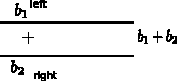
\includegraphics{diagrams/thesis/sum-two-wires.pdf}
}
\end{center}
\begin{center}
\scalebox{0.95}{
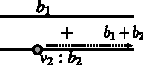
\includegraphics{diagrams/thesis/sum-two-wires-right-value.pdf}
}
\end{center}
\end{multicols}

\item Associativity is implicit in the graphical language. Three parallel
  wires represent {{b1*(b2*b3)}} or {{(b1*b2)*b3}}, based on the context.
\begin{center}
\scalebox{0.95}{
%%subcode-line{pdfimage}[diagrams/thesis/associate.pdf]
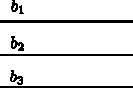
\includegraphics{diagrams/thesis/assoc.pdf}
}
\end{center}

\item Commutativity is represented by crisscrossing wires.
\begin{multicols}{2}
\begin{center}
\scalebox{0.95}{
%%subcode-line{pdfimage}[diagrams/thesis/swap-pair.pdf]
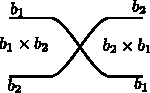
\includegraphics{diagrams/thesis/swap_times.pdf}
}
\end{center}
\begin{center}
\scalebox{0.95}{
%%subcode-line{pdfimage}[diagrams/thesis/swap-sum.pdf]
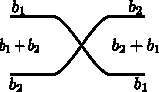
\includegraphics{diagrams/thesis/swap_plus.pdf}
}
\end{center}
\end{multicols}

By visually tracking the flow of particles on the wires, one can
verify that the expected types for commutativity are satisfied.

\begin{multicols}{2}
\begin{center}
\scalebox{0.95}{
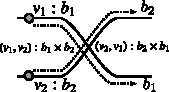
\includegraphics{diagrams/thesis/swap_times_value.pdf}
}
\end{center}
\begin{center}
\scalebox{0.95}{
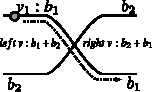
\includegraphics{diagrams/thesis/swap_plus_value.pdf}
}
\end{center}
\end{multicols}


\item The morphisms that witness that {{0}} and {{1}} are the additive and
  multiplicative units are represented as shown below. Note that since there
  is no value of type 0, there can be no particle on a wire of type {{0}}.
  Also since the monoidal units can be freely introduced and eliminated, in
  many diagrams they are omitted and dealt with explicitly only when they are
  of special interest.
\begin{multicols}{2}
\begin{center}
\scalebox{0.95}{
%%subcode-line{pdfimage}[diagrams/thesis/identr1.pdf]
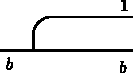
\includegraphics{diagrams/thesis/uniti.pdf}
}
\end{center}
\begin{center}
\scalebox{0.95}{
%%subcode-line{pdfimage}[diagrams/thesis/identl1.pdf]
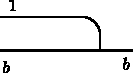
\includegraphics{diagrams/thesis/unite.pdf}
}
\end{center}  
\end{multicols}
\begin{multicols}{2}
\begin{center}
\scalebox{0.95}{
%%subcode-line{pdfimage}[diagrams/thesis/identr0.pdf]
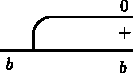
\includegraphics{diagrams/thesis/zeroi.pdf}
}
\end{center}
\columnbreak
\begin{center}
\scalebox{0.95}{
%%subcode-line{pdfimage}[diagrams/thesis/identl0.pdf]
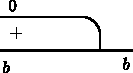
\includegraphics{diagrams/thesis/zeroe.pdf}
}
\end{center}
\end{multicols}

\item Finally, distributivity and factoring are represented using the dual
  boxes shown below:
\begin{multicols}{2}
\begin{center}
  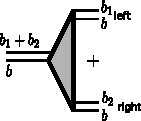
\includegraphics{diagrams/thesis/dist.pdf}
\end{center}
\begin{center}
  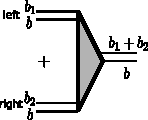
\includegraphics{diagrams/thesis/factor.pdf}
\end{center}
\end{multicols}

Distributivity and factoring are interesting because they represent
interactions between sum and pair types. Distributivity should
essentially be thought of as a multiplexer that redirects the flow of
{{v:b}} depending on what value inhabits the type {{b1+b2}}, as shown
below. Factoring is the corresponding adjoint operation.

\begin{multicols}{2}
\begin{center}
  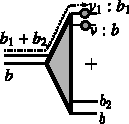
\includegraphics{diagrams/thesis/dist-wire-value1.pdf}
\end{center}
\begin{center}
  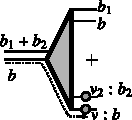
\includegraphics{diagrams/thesis/dist-wire-value2.pdf}
\end{center}
\end{multicols}

\item Composition TODO.

  \begin{multicols}{2}
\dgm{c1c2_par_sum}
\dgm{c1c2_par_times}
  \end{multicols}
\dgm{c1c2_seq}    

\end{itemize}

\noindent 
\textit{Example.}  We use the type {{bool}} as a shorthand to denote
the type {{1+1}} and use {{left ()}} to be {{true}} and {{right ()}}
to be {{false}}. The following combinator is represented by the given
diagram:

{{c : b * bool <-> b + b}}

{{c = swap* (;) dist (;) (identl* (+) identl*)}}

\begin{center}
\scalebox{0.95}{
%%subcode-line{pdfimage}[diagrams/thesis/example1-crop.pdf]
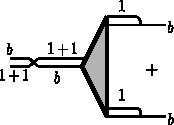
\includegraphics{diagrams/thesis/example1.pdf}
}
\end{center}

%%%%%%%%%%%%%%%%%%%
\subsection{Semantics}

The operational semantics of {{Pi}} is summarized below (also see
\cite{infeffects}).  The semantics of the primitive combinators is
given by the following single-step reductions below. Since there are
no values of type {{0}}, the rules omit the impossible cases:
\begin{scriptsize}
%subcode{opsem} include main
%! columnStyle = rlcl
% swap+ & (left v) &|-->& right v
% swap+ & (right v) &|-->& left v 
% assocl+ & (left v1) &|-->& left (left v1)
% assocl+ & (right (left v2)) &|-->& left (right v2)
% assocl+ & (right (right v3)) &|-->& right v3 
% assocr+ & (left (left v1)) &|-->& left v1
% assocr+ & (left (right v2)) &|-->& right (left v2)
% assocr+ & (right v3) &|-->& right (right v3)
% identl* & ((), v) &|-->& v 
% identr* & v &|-->& ((), v) 
% swap* & (v1, v2) &|-->& (v2, v1) 
% assocl* & (v1, (v2, v3)) &|-->& ((v1, v2), v3) 
% assocr* & ((v1, v2), v3) &|-->& (v1, (v2, v3)) 
% dist & (left v1, v3) &|-->& left (v1, v3)
% dist & (right v2, v3) &|-->& right (v2, v3)
% factor & (left (v1, v3)) &|-->& (left v1, v3) 
% factor & (right (v2, v3)) &|-->& (right v2, v3)   
\end{scriptsize}
The operational semantics of the closure conditions are presented in
the usual big-step style.
\begin{scriptsize}
%subcode{proof} include main
%@ ~
%@@ id v |--> v 
%
%@ c{dagger} v1 |--> v2
%@@ (sym c) v1 |--> v2
%
%@ c1  v1 |--> v
%@ c2  v |--> v2
%@@ (c1(;)c2)  v1 |--> v2
%---
%@ c1  v1 |--> v2
%@@ (c1 (+) c2)  (left v1) |--> left v2
%
%@ c2  v1 |--> v2
%@@ (c1 (+) c2)  (right v1) |--> right v2
%---
%@ c1  v1 |--> v3
%@ c2  v2 |--> v4
%@@ (c1 (*) c2)  (v1, v2) |--> (v3, v4)
\end{scriptsize}

The type safety of {{Pi}} follows directly from the correspondence
between inductive definitions of the types and the big-step
semantics. Previous work also established the following properties:

\begin{proposition}[Strong Normalizing]
\label{prop:termination-pi} 
{{Pi}} computations always terminate.  

{{forall. c:b1<->b2, v:b1, exists v':b2.}}  
{{c v |--> v'}}
\end{proposition}

\begin{proposition}[Logical Reversibility]
\label{prop:logrev}
{{c v |--> v'}} iff 
{{ c{dagger} v' |--> v}}
\end{proposition}

%%%%%%%%%%%%%%%%%%%
\subsection{Constructions}

\paragraph*{Booleans and Conditionals.} 
Given any combinator {{c : b <-> b}} we can construct a combinator called
{{if_c : bool*b <->bool*b}} in terms of {{c}}, where {{if_c}} behaves like a
one-armed $\mathit{if}$-expression. If the supplied boolean is {{true}} then
the combinator {{c}} is used to transform the value of type~{{b}}. If the
boolean is {{false}}, then the value of type {{b}} remains unchanged. We can
write down the combinator for {{if_c}} in terms of {{c}} as 
{{ dist (;) ((id (*) c) (+) id) (;) factor }}.

\noindent The diagram below shows the input value of type {{(1+1)*b}}
processed by the distribute operator {{dist}}, which converts it into a value
of type {{(1*b)+(1*b)}}. In the {{left}} branch, which corresponds to the
case when the boolean is {{true}} (i.e. the value was {{left ()}}), the
combinator~{{c}} is applied to the value of type~{{b}}. The right branch
which corresponds to the boolean being {{false}} passes along the value of
type {{b}} unchanged.

\begin{center}
\scalebox{1.0}{
%%subcode-line{pdfimage}[diagrams/if_c.pdf]
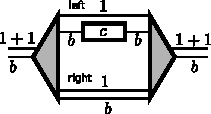
\includegraphics{diagrams/thesis/cnot.pdf}
}
\end{center}

The combinator {{if_{not} }} has type {{bool*bool<->bool*bool}} and
negates its second argument if the first argument is {{true}}. This
gate {{if_{not} }} is often referred to as the {{cnot}} gate. An
equivalent construction that is useful is {{else_{not} }} where we
negate the second argument only if the first is {{false}}. 

Similarly, we can iterate the construction of {{if_c}} to check several
bits. The gate {{if_{cnot} }}, which we may also write as {{if^2_{not} }},
checks two booleans and negates the result wire only if they are both
{{true}}. The gate {{if^2_{not} }} is well known as the Toffoli gate and is a
universal reversible gate. We can generalize this construction to
{{if^n_{not} }} which checks {{n}} bits and negates the result wire only if
they are all {{true}}.

\paragraph*{Cloning.}
Although cloning is generally not allowed in reversible languages, it is
possible at the cost of having additional constant inputs. For example,
consider the gate {{else_{not} }}. Generally, the gate maps
{{(false,a)}} to {{(false,not a)}} and {{(true,a)}} to {{(true,a)}}. Focusing
on the cases in which the second input is {{true}}, we get that the gate maps
{{(false,true)}} to {{(false,false)}} and {{(true,true)}} to {{(true,true)}},
i.e., the gate clones the first input. A circuit of {{n}} parallel
{{else_{not} }} gates can hence clone {{n}} bits.  They also consume {{n}}
{{true}} inputs in the process.  Let us call this construction
{{clone^n_{bool} }}.

%%%%%%%%%%%%%%%%%
\subsection{Categorical Structure}

For the purpose of establishing equivalence of morphisms in the
categorical presentation we use the following notion of equality:

\begin{lemma}[{{c1  = c2}}]
We say {{c1 = c2}} if {{c1:b1<->b2}} and {{c2:b1<->b2}} and for all
{{v1:b}}, we have {{c1 v1 |--> v2}} iff {{c2 v1 |--> v2}} and {{v2:b2}}.
\end{lemma}

We present the categorical structure with minimum commentary. More
details may be found in excellent references such as Barr and Wells
[CITE] and Selinger \cite{springerlink:10.1007/978-3-642-12821-94}.

\begin{lemma}[{{Pi}} is a category]
  The category {{Pi}} has the types {{b}} as objects and equivalence
  classes of well-typed combinators {{b1<->b2}} as morphisms. One can
  check:
  \begin{enumerate}
  \item Every object {{b}} has an identity morphism {{id : b <->b}}.
  \item Composition {{g (o) f}} of morphisms {{f:b1 <->b2}} and
    {{g:b2<->b3}} is given by sequencing {{f (;) g}}. 
  \item Associativity of composition follows from operational
    equivalence of {{f(;)(g(;)h)}} and {{(f(;)g)(;)h}} (where
    {{h:b3<->b4}}). 

    Assuming {{v1:b1}}, {{v2:b2}}, {{v3:b3}}, {{v4:b4}},
    {{f~v1|-->v2}}, {{g v2 |--> v3}} and {{h~v3 |--> v4}}, one can
    check:

\vspace{-20pt}
    \begin{multicols}{2}
      \begin{scriptsize}
        
%subcode{proof} include main
%@@ f v1 |--> v2
%@ g v2 |--> v3
%@ h v3 |--> v4
%@@ g (;) h  v2 |--> v4
%@@@ f (;) (g (;) h) v1 |--> v4
~
%subcode{proof} include main
%@ f v1 |--> v2
%@ g v2 |--> v3
%@@ f (;) g v1 |--> v3
%@@ h v3 |--> v4
%@@@ (f (;) g) (;) h v1 |--> v4

      \end{scriptsize}
    \end{multicols}

  \item Composition respects identity: {{id (;) f = f}} and {{g(;)id=g}}.
  \end{enumerate}
\end{lemma}

\begin{lemma}[Dagger]
  {{Pi}} is a dagger category, where every morphism {{f : b1<->b2}}
  has the adjoint {{f^{dagger}:b2 <->b1}}. The following properties
  hold (where {{g : b2 <-> b3}}): 
  \begin{enumerate}
  \item {{id^{dagger} = id : b <-> b}}.
  \item {{(f (;) g)^{dagger} = g^{dagger} (;) f^{dagger}: b3 <-> b1}}.
  \item {{f^{dagger dagger} = f : b1 <-> b2}}.
  \end{enumerate}
\end{lemma}

\begin{lemma}[Symmetric Monoidal (+, 0)]
  {{Pi}} is a symmetric monoidal category with tensor {{+}} and
  monoidal unit {{0}}. The monoidal operation on morphisms is the
  additive composition of combinators {{c1 (+) c2}}.

  \begin{proof}
    To establish that category is monoidal one must show isomorphisms
    \begin{enumerate}
    \item {{b1 + (b2 + b3) <-> (b1 +b2) + b3}} given by {{assocl+}}.
    \item {{0 + b <-> b}} given by {{zeroe}}.
    \item {{b + 0 <-> b}} given by {{swap+ (;) zeroe}}.
    \item We need to check that {{+}} is a bifunctor. 
      \begin{enumerate}
      \item {{id_{b1<->b1}(+)id_{b2<->b2} = id_{b1+b2<->b1+b2} }}.
      \item {{(f(+)g)(;)(j(+)k) = (f (;) j) (+) (g (;) k)}}.
      \end{enumerate}
    \item We need to check the naturality of {{assocl+}}, {{zeroe}} and
      {{swap+(;)zeroe}}.
      \begin{enumerate}
      \item {{assocl+ (;) ((f (+)g) (+) h) = (f (+)(g (+) h)) (;) assocl+}}.
      \item {{zeroe (;) f = (id (+) f) (;) zeroe}}.
      \item {{(swap+ (;) zeroe) (;) f = (f (+) id) (;) (swap+ (;) zeroe)}}.
      \end{enumerate}
    \item Satisfy certain coherence conditions which are usually
      called the ``pentagon'' and ``triangle'' axioms (see Sec 3.1
      \cite{springerlink:10.1007/978-3-642-12821-94})
    \end{enumerate}

    The last three points require checking equality of combinators by
    writing out their derivation trees as we did in the case of
    associativity of sequential composition. To show symmetry, we need
    a braiding operation {{b1+b2 <-> b2+b1}} which is given by
    {{swap+}} (see Sec. 3.3 and 3.5
    \cite{springerlink:10.1007/978-3-642-12821-94}).

    \begin{enumerate}
    \item The braiding must satisfy two ``hexagon'' axioms.
    \item The braiding is self inverse,
      {{swap+_{b1+b2}=(swap+_{b2+b1})^{dagger} }}.
    \end{enumerate}


  \end{proof}

\end{lemma}

\begin{lemma}[Symmetric Monoidal {{(*, 1)}}]
  {{Pi}} is a symmetric monoidal category over the tensor {{*}} and
  unit {{1}}. The details mirror those of the {{(0, +)}} monoid.
\end{lemma}

\noindent
Some technical and pedantic comments are due at this point. 

\begin{itemize}
\item We have established the categorical structure of {{Pi}} as a
  dagger symmetric monoidal category with two monoidal structures,
  {{(0, +)}} and {{(*, 1)}}. In Sec. \ref{sec:int} we will see that a
  {{trace}} operator can be admitted in this category without any
  change of expressiveness.

\item To be pedantic, what we have shown is that the ``term model'' of
  {{Pi}} that follows from the extensional operational equality of
  combinators has the requisite categorical structure. A consequence
  is that the ``wiring diagrams'' of {{Pi}} correspond closely with ``string
  diagrams'' developed for categories.

  To establish the later rigorously, we will need to show when it is
  valid to slide one wire over the other and that equivalent diagrams
  for syntactically different combinators such as
  {{(f(+)g)(;)(j(+)k)}} and {{(f(;)j)(+)(g(;)k)}} do respect
  operational equivalence.  We don't formalize the graphical notation
  in this work. Joyal et. al's work on ``planar isotopy'' and
  Selinger's survey \cite{springerlink:10.1007/978-3-642-12821-94}
  show how this has been addressed before in the categorical
  setting. In the absence of any prior knowledge of category theory
  however, our wiring diagrams may be read as the ``flow of types'' in
  a combinator-circuit.

\item By definition, in {{Pi}} every morphism is an isomorphism --
  this makes {{Pi}} a groupoid.

\item The category {{Pi}} has no initial and terminal objects. The
  objects {{0}} and {{1}} would be initial and terminal if we admitted
  all functions (as in the category {{CatSet}}).

\item The category {{Pi}} has neither categorical products, nor
  categorical co-products, i.e. {{*}} and {{+}} are merely monoidal
  tensors. This follows from the fact that injection and projection
  maps are not isomorphisms.
\end{itemize}

While we don't do so in this work, if we extend {{Pi}} with products
and co-products (say through the addition of information effects) it
is conceivable that part of its structure collapses. This sort of
collapse, while catastrophic for algebraic structures (effectively
trivializing them), still retains some interest in computing, because
in computing we are interested in the specific operational nature (the
computational content, so to speak) of the morphisms. Anecdotal evidence
follows from the fact several real-world programming language have
inconsistent type systems. blah blah blah...

%%%%%%%%%%%%%
\subsection{Small Step Semantics}

The reductions for the primitive isomorphisms above are exactly the same as
have been presented before~\cite{infeffects}. The reductions for the closure
combinators are however presented in a small-step operational style using the
following definitions of evaluation contexts and machine states:

\begin{scriptsize}
%subcode{bnf} include main
% Combinator Contexts, C = [] | Fst C c | Snd c C 
%                  &|& LeftT C c v | RightT c v C 
%                  &|& LeftP C c | RightP c C 
% Machine states = <c, v, C> | {[c, v, C]}
% Start state = <c, v, []> 
% Stop State = {[c, v, []]}
\end{scriptsize}
The machine transitions below track the flow of particles through a
circuit. The start machine state, , denotes the
particle~{{v}} about to be evaluated by the circuit {{c}}. The end
machine state, {{[c, v, [] ]}}, denotes the situation where the particle
{{v}} has exited the circuit {{c}}.

\begin{scriptsize}
%subcode{opsem} include main
%! columnStyle = rclr
% <iso, v, C> &|-->& {[iso, v', C]} & (1)
% & & where iso v |--> v' &
% <c1(;)c2, v, C> &|-->& <c1, v, Fst C c2> & (2) 
% {[c1, v, Fst C c2]} &|-->& <c2, v, Snd c1 C> & (3) 
% {[c2, v, Snd c1 C]} &|-->& {[ c1(;)c2, v, C ]} & (4) 
% <c1(+)c2, left v, C> &|-->& <c1, v, LeftP C c2> & (5) 
% {[ c1, v, LeftP C c2 ]} &|-->& {[c1 (+) c2, left v, C ]} & (6)
% <c1(+)c2, right v, C> &|-->& <c2, v, RightP c1 C> & (7)
% {[ c2, v, RightP c1 C ]} &|-->& {[c1 (+) c2, right v, C ]} & (8)
% <c1(*)c2, (v1, v2), C> &|-->& <c1, v1, LeftT C c2 v2> & (9)
% {[ c1, v1, LeftT C c2 v2 ]} &|-->& <c2, v2, RightT c1 v1 C> & (10) 
% {[ c2, v2, RightT c1 v1 C ]} &|-->& {[ c1 (*) c2, (v1, v2), C ]} & (11)
\end{scriptsize}
Rule (1) describes evaluation by a primitive isomorphism. Rules (2), (3) and
(4) deal with sequential evaluation. Rule (2) says that for the value {{v}}
to flow through the sequence {{c1 (;) c2}}, it should first flow through
{{c1}} with {{c2}} pending in the context ({{Fst C c2}}). Rule (3) says the
value {{v}} that exits from {{c1}} should proceed to flow
through~{{c2}}. Rule (4) says that when the value {{v}} exits {{c2}}, it also
exits the sequential composition {{c1(;)c2}}. Rules (5) to (8) deal with 
{{c1 (+) c2}} in the same way. In the case of sums, the shape of the value,
i.e., whether it is tagged with {{left}} or {{right}}, determines whether
path {{c1}} or path {{c2}} is taken. Rules (9), (10) and (11) deal with 
{{c1 (*) c2}} similarly. In the case of products the value should have the
form {{(v1, v2)}} where {{v1}} flows through {{c1}} and {{v2}} flows through
{{c2}}. Both these paths are entirely independent of each other and we could
evaluate either first, or evaluate both in parallel. In this presentation we
have chosen to follow {{c1}} first, but this choice is entirely arbitrary.

The interesting thing about the semantics is that it represents a reversible
abstract machine. In other words, we can compute the start state from the
stop state by changing the reductions {{|-->}} to run backwards
{{<--|}}. When running backwards, we use the isomorphism represented by a
combinator {{c}} in the reverse direction, i.e., we use the adjoint
{{c{dagger}}}.

\begin{proposition}[Correspondence]
  Evaluation in the small-step evaluator corresponds to evaluation in
  the natural semantics.

  {{c v |--> v'}} iff {{<c, v, []> |-->* [c', v', [] ]}}
\end{proposition}
\begin{proof}
  To prove the above, we first show that a more general lemma holds,
  namely that: {{c v |--> v'}} iff {{<c, v, C> |-->* [c', v', C ]}}.

  To show the left-to-right direction we proceed by induction on the
  derivation of {{c v |--> v'}}. In the case of primitive isomorphisms
  the condition holds trivially. In the case of composition, we work
  out the case of {{c1+c2}} as an example. Given {{c1 +c2 v |--> v'}}
  we have to show that there is a small step derivation sequence that
  matches it. Here {{v:b1+b2}} can be of the form {{left v1}} or
  {{right v2}}. Assuming {{left v1}}, we have: 

%subcode{proof} include main
%@ c1 v1 |--> v1' ==> <c1, v1, C'> |-->* {[c1',v1',C']}
%@@ c1+c2 (left v1) |--> left v1' ==> ? 

Choosing {{C' =Lft c2 C}}, we have the required derivation sequence: 
{{ <c1+c2, left v1, C> |--> <c1,v1,LeftP c2 C> |-->* {[c1',v1', LeftP c2 C]} |--> {[c1'+c2,left v1',C]} }}. The proof follows similarly for the {{right v2}} case.  

To show the right-to-left direction we proceed by induction of the
sequence of {{|-->*}} derivations. Again the case for primtive
isomorphisms follows trivially. Taking the case of {{c1+c2}} we are
required to show that given a sequence 
{{<c1+c2,v,C> |-->* {[c', v', C]} }} there is a derviation tree for
{{c1+c2 v |--> v'}}. In the case that {{v:v1+b2}} has the form
{{left~v1}}, this follows by observing that the given sequence must have the form
{{ <c1+c2, left v1, C> |--> <c1,v1,LeftP c2 C> |-->* {[c1',v1', LeftP c2 C]} |--> {[c1'+c2,left v1',C]} }}. 
For the strictly smaller inner subsequence by induction we have
{{c1~v1 |--> v1'}} which lets us complete the derivation of
{{c1+c2~(left v1) |--> left v1'}}. The {{right v2}} follows similarly. 

\end{proof}

%%%%%%%%%%%%%%%%%%%%%%%%%%%%%%%%%%%%%%%%%%%%%%%%%%%%%%%%%%%%%%%%%%%%%%%%
\begin{small}
\bibliographystyle{abbrvnat}
\bibliography{cites}
\end{small}

\end{document}

%%%%%%%%%%%%%%%%%%%%%%%%%%%%%%%%%%%%%%%%%%%%%%%%%%%%%%%%%%%%%%%%%%%%%%%%
